\section{Регулятор с качественной экспоненциальной устойчивостью}
Рассмотрим систему: 
\begin{equation}
    \dot{x} = Ax + Bu
\end{equation}
где 
\begin{equation}
    \begin{array}{cc}
        A = \begin{bmatrix}
            8 & 1 & 11 \\ 
            4 & 0 & 4 \\
            -4 & -3 & -7
        \end{bmatrix}, &
        B = \begin{bmatrix}
            -1 \\ -3 \\ 3
        \end{bmatrix}
    \end{array}
\end{equation}


Для определения управляемости собственных чисел рассмотрим вещественную Жорданову форму системы: 
\begin{equation}
    \dot{\hat{x}} = P^{-1}AP\hat{x} + P^{-1}Bu
\end{equation}
Где $P$ -- матрица собственных векторов матрицы $A$, а $\hat{x} = P^{-1}x$.
\begin{equation}
    A_j = \begin{bmatrix}
        -3  & 0  & 0 \\ 
        0  & 2  & -2 \\ 
        0  & 2  & 2 \\ 
    \end{bmatrix}\quad
    P = \begin{bmatrix}
        -1  & -2.12  & 0.71 \\ 
        0  & -1.41  & 0 \\ 
        1  & 1.41  & 0 \\ 
    \end{bmatrix}\quad 
    B_j = \begin{bmatrix}
        0 \\ 
        2.12 \\ 
        4.95 \\ 
    \end{bmatrix}
\end{equation}

Таким образом, последнее собственное число $\lambda_3 = -3$ не является управляемым. Соответственно, система не является полностью управляемой. 
Но, так как данное собственное число располагается в левой полуплоскости, то есть является устойчивым, то система является стабилизируемой. 

\subsection{Синтез регулятора}
Зададимся значением $\beta = -4$ как средним значением поведения траектории системы 
и параметром $r = 2$, характеризующим разброс разброс поведения траектории 
относительно значения $\beta$.

С помощью матричного уравнения Риккати синтезируем регулятор $K$: 
\begin{eqnarray}
    (A - Bk - \beta I)^TP(A - Bk - \beta I) - r^2P = -Q, & K = (-R + B^T PB)^{-1}B^TP(A - \beta I)
\end{eqnarray}
для каждой из пар значений $Q$ и $R$:
\begin{enumerate}
    \item $Q = I, R = 1$
    \item $Q = I, R = 0$ 
    \item $Q = 0, R = 1$
    \item $Q = 0, R = 0$
\end{enumerate}

Полученные значения матрицы $K_i$:
\begin{equation}
    \begin{array}{cccc}
        K_1 = \begin{bmatrix}
            -3.10  & 0.98  & -3.10 \\ 
        \end{bmatrix} \\
        K_2 = \begin{bmatrix}
            -3.16  & 1.00  & -3.16 \\ 
        \end{bmatrix} \\
        K_3 = \begin{bmatrix}
            -3.29  & 1.14  & -3.29 \\ 
        \end{bmatrix} \\ 
        K_4 = \begin{bmatrix}
            -4.29  & 1.00  & -4.29 \\
        \end{bmatrix}
    \end{array}
\end{equation}
Для каждой системы, замкнутой регулятором $K_i$, найдем собственные числа матрицы $A - BK_i$: 
\begin{equation}
    \begin{array}{cccc}
        \sigma_1 = \begin{bmatrix}
            -2.57 + 0.58j \\ 
            -2.57 - 0.58j \\ 
            -3.00 \\ 
        \end{bmatrix} & 
        \sigma_2 = \begin{bmatrix}
            -3.00 \\ 
            -2.32 \\ 
            -3.00 \\ 
        \end{bmatrix} &
        \sigma_3 = \begin{bmatrix}
            -2.62 + 1.96j \\ 
            -2.62 - 1.96j \\ 
            -3.00 \\ 
        \end{bmatrix} &
        \sigma_4 = \begin{bmatrix}
            -3.00 \\ 
            -3.00 \\ 
            -4.58 \\ 
        \end{bmatrix}
    \end{array}
\end{equation}

Построим окружность на комплексной плоскости с центром в точке $(\beta, 0)$ и радиусом $r$, 
на этой же плоскости разместим собственные числа системы, замкнутой по регулятору $K_i$. 
Полученные графики представлены на рисунке \ref{fig:task3_eigs1} -- \ref{fig:task3_eigs4}.

\begin{figure}[ht!]
    \centering
    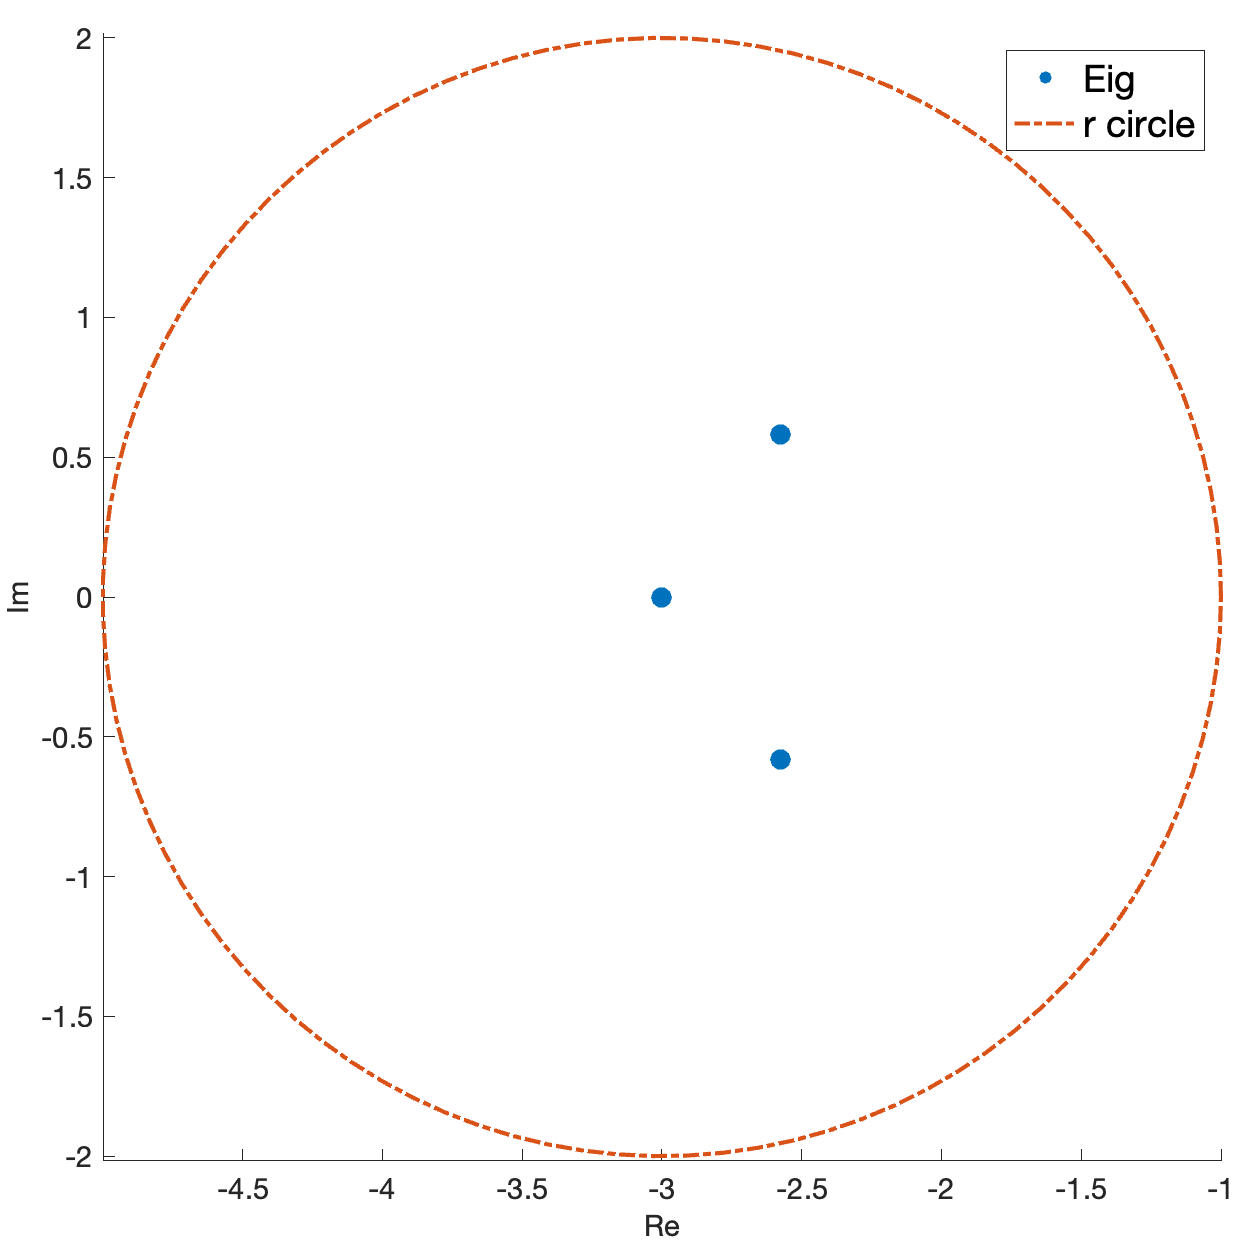
\includegraphics[width=0.7\textwidth]{media/plots/task3_eigs_1.png}
    \caption{Собственные числа системы, замкнутой по регулятору $K_1$}
    \label{fig:task3_eigs1}
\end{figure}
\begin{figure}[ht!]
    \centering
    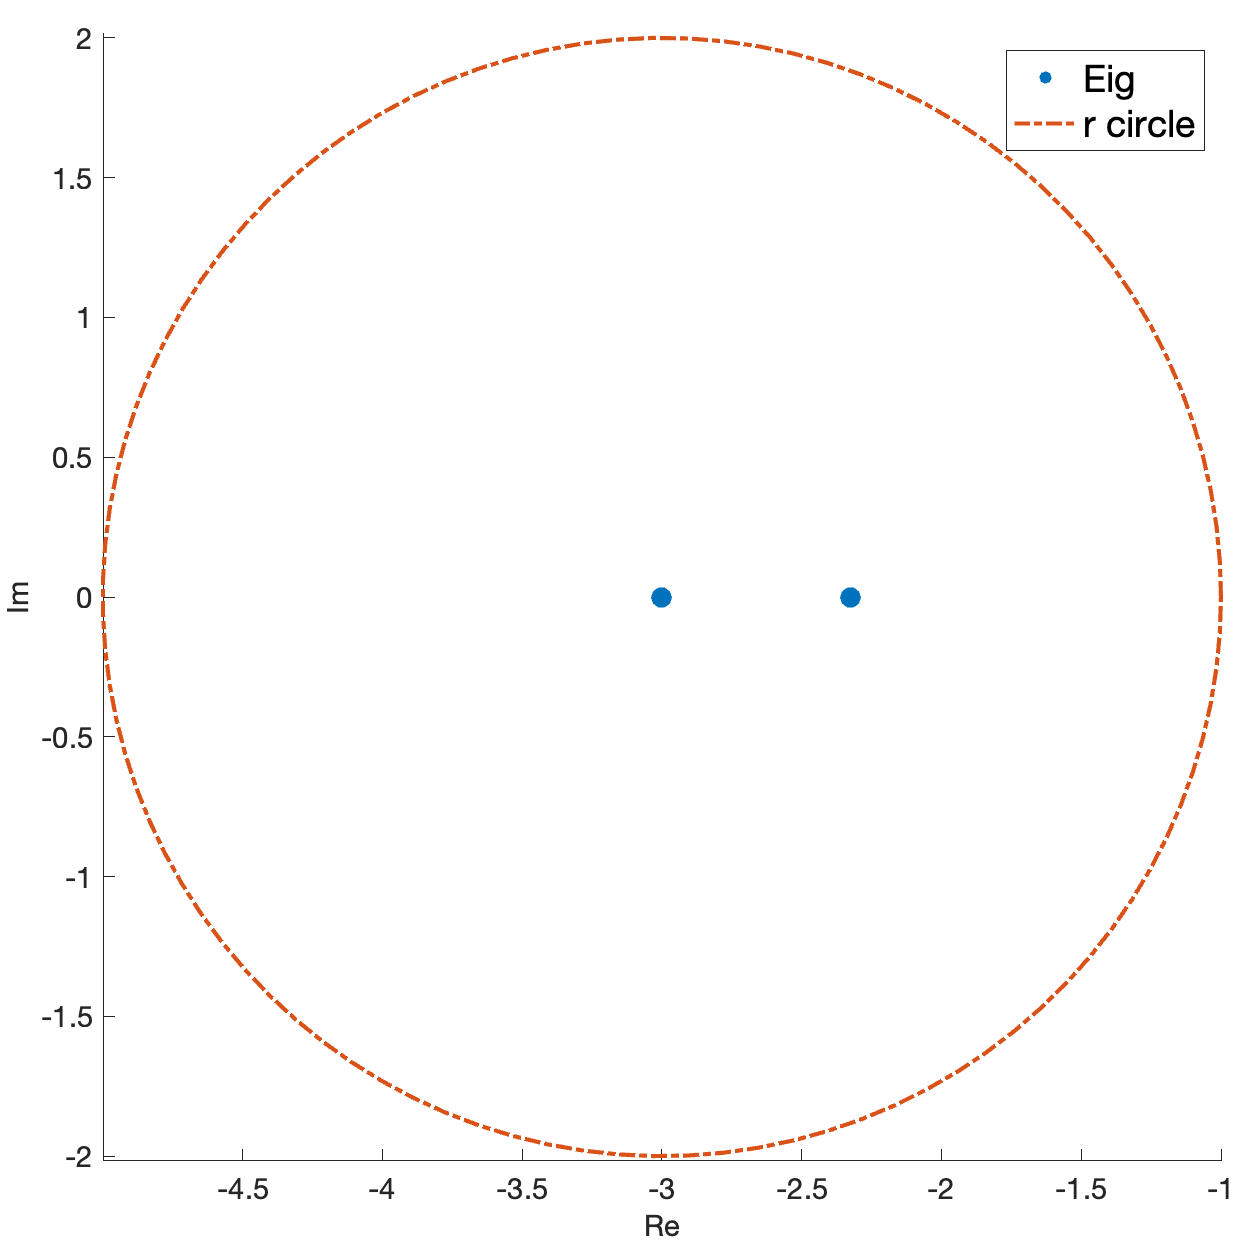
\includegraphics[width=0.7\textwidth]{media/plots/task3_eigs_2.png}
    \caption{Собственные числа системы, замкнутой по регулятору $K_2$}
    \label{fig:task3_eigs2}
\end{figure}
\begin{figure}[ht!]
    \centering
    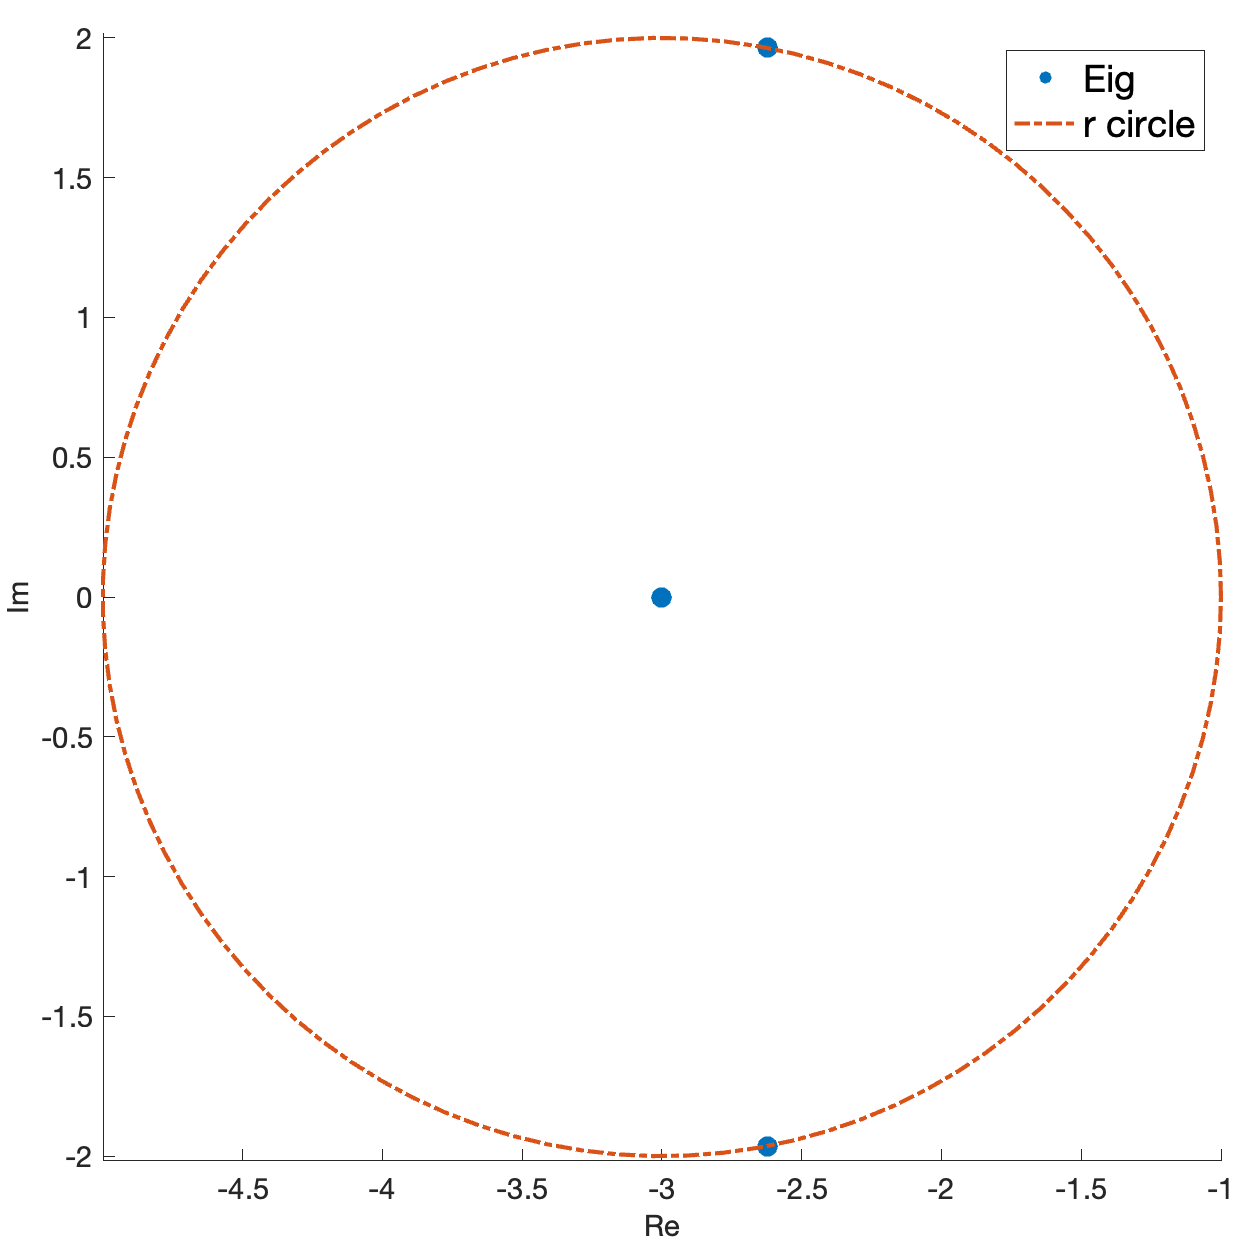
\includegraphics[width=0.7\textwidth]{media/plots/task3_eigs_3.png}
    \caption{Собственные числа системы, замкнутой по регулятору $K_3$}
    \label{fig:task3_eigs3}
\end{figure}
\begin{figure}[ht!]
    \centering
    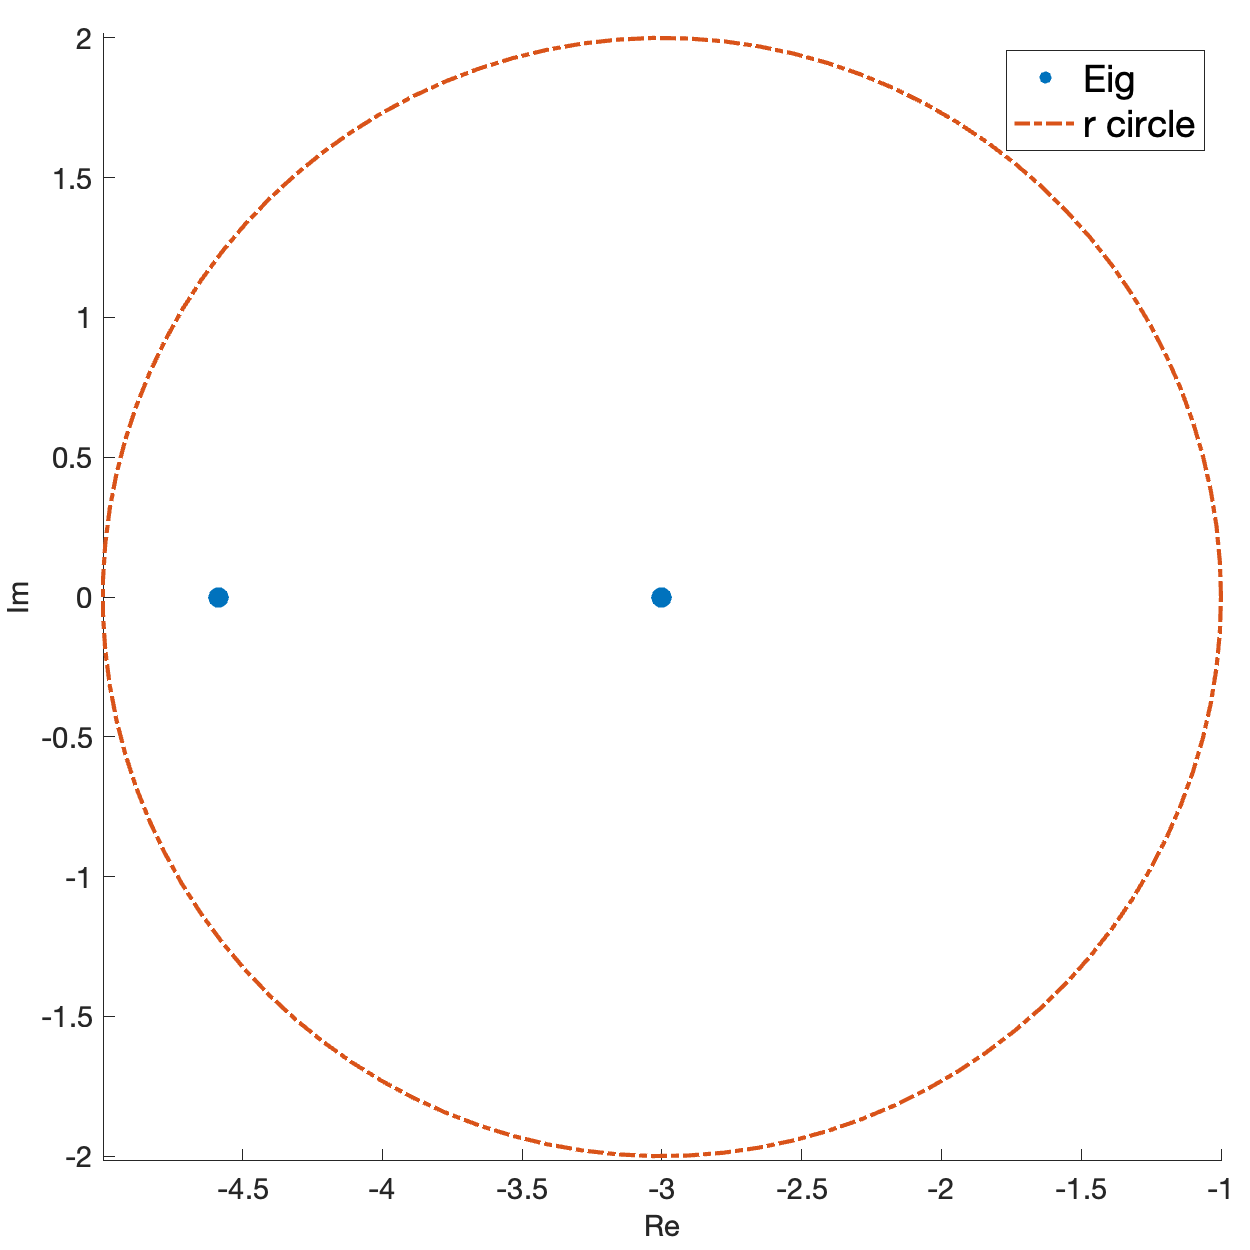
\includegraphics[width=0.7\textwidth]{media/plots/task3_eigs_4.png}
    \caption{Собственные числа системы, замкнутой по регулятору $K_4$}
    \label{fig:task3_eigs4}
\end{figure}

Видно, что во всех случаях полученные собственные числа замкнутой регулятором 
системы располагаются внутри окружности, что подтверждает, что полученные регуляторы 
обеспечивают качественную экспоненциальную устойчивость системы. 

\subsection{Моделирование}
Проведем моделирование систем, замкнутых по регуляторам $K_i$. 

Для системы с регулятором $K_1$ результаты моделирования представлены на рисунке \ref{fig:task3_x} 
(состояние системы) и \ref{fig:task3_1_u} (управляющее воздействие).

\begin{figure}[ht!]
    \centering
    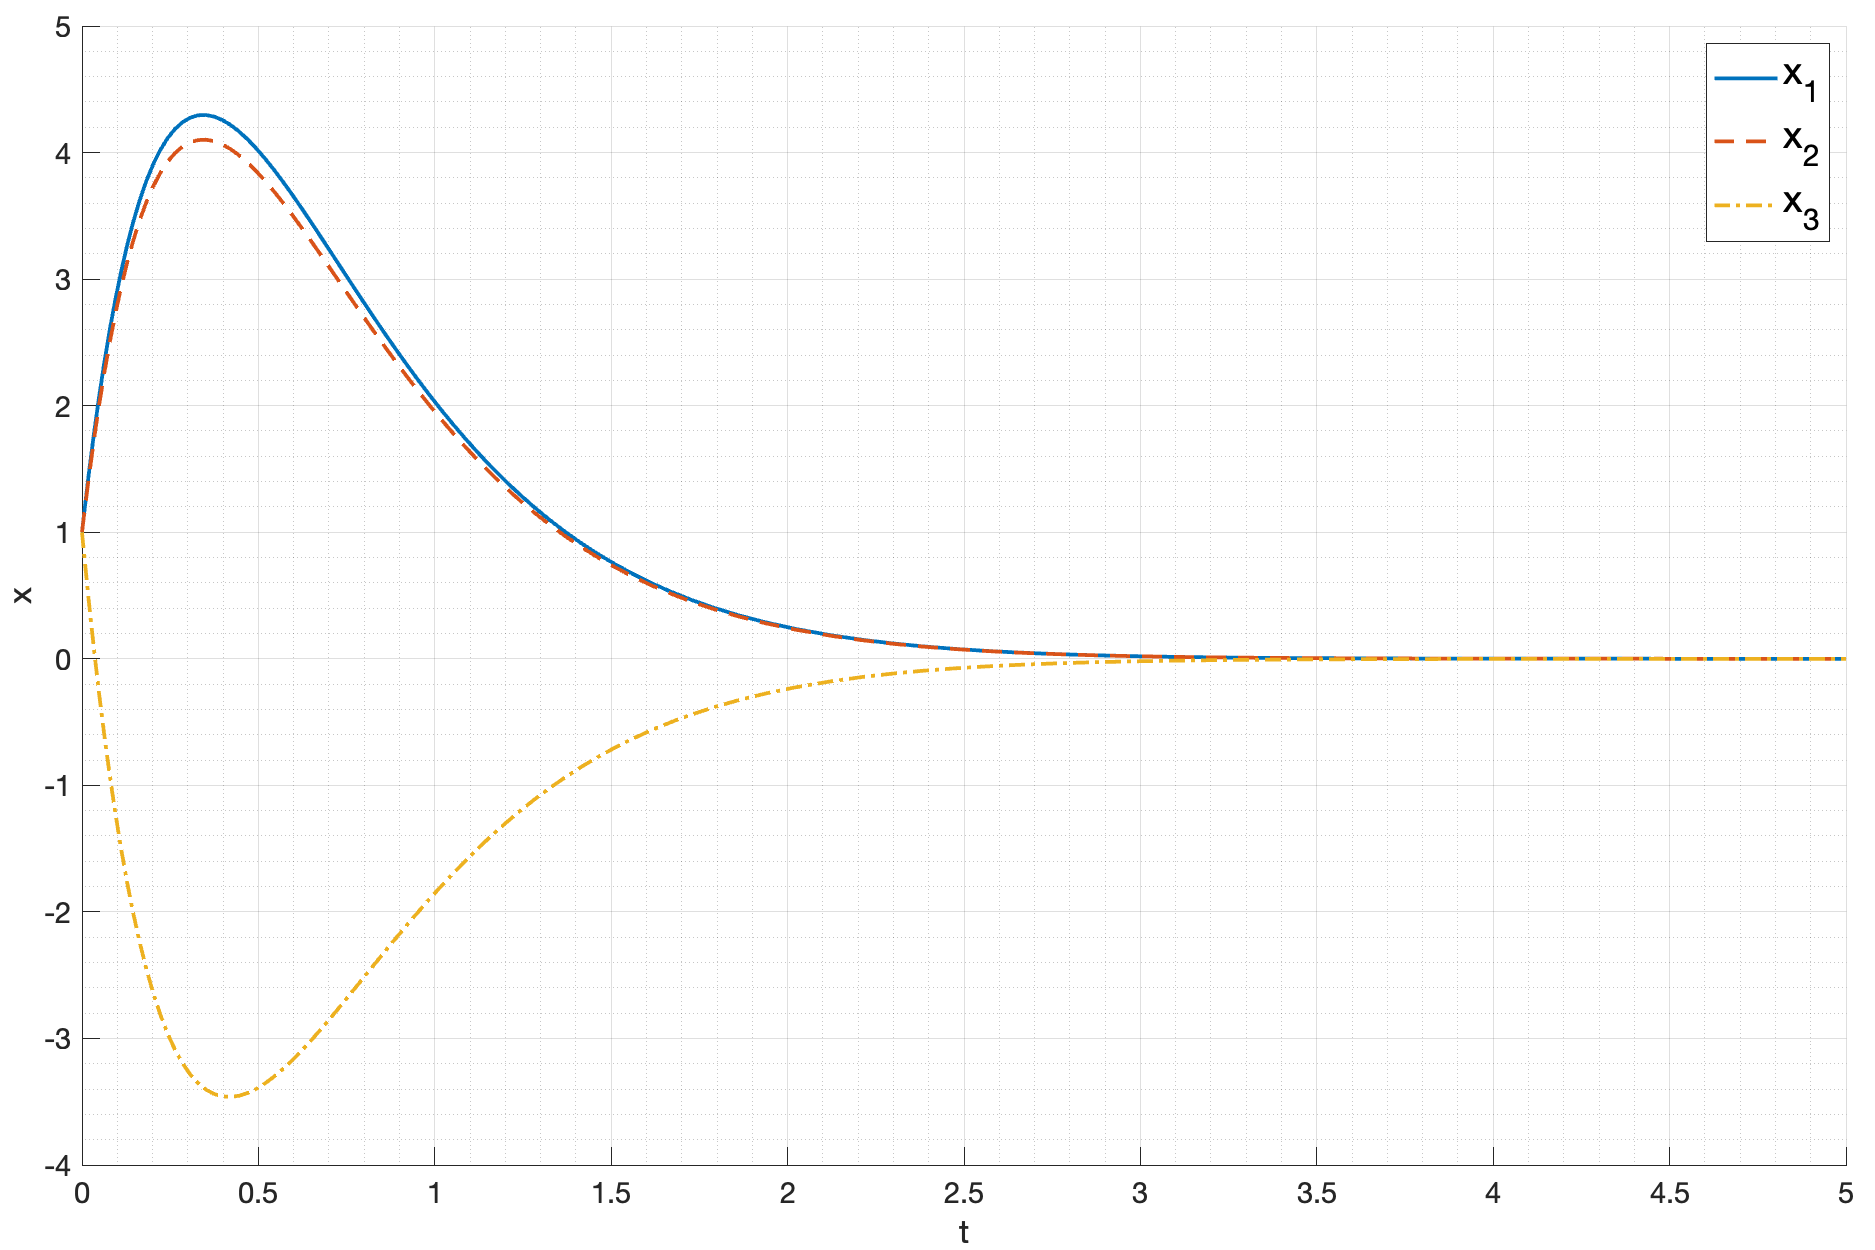
\includegraphics[width=\textwidth]{media/plots/task3_1_x.png}
    \caption{Состояние системы с регулятором $K_1$}
    \label{fig:task3_1_x}
\end{figure}
\begin{figure}[ht!]
    \centering
    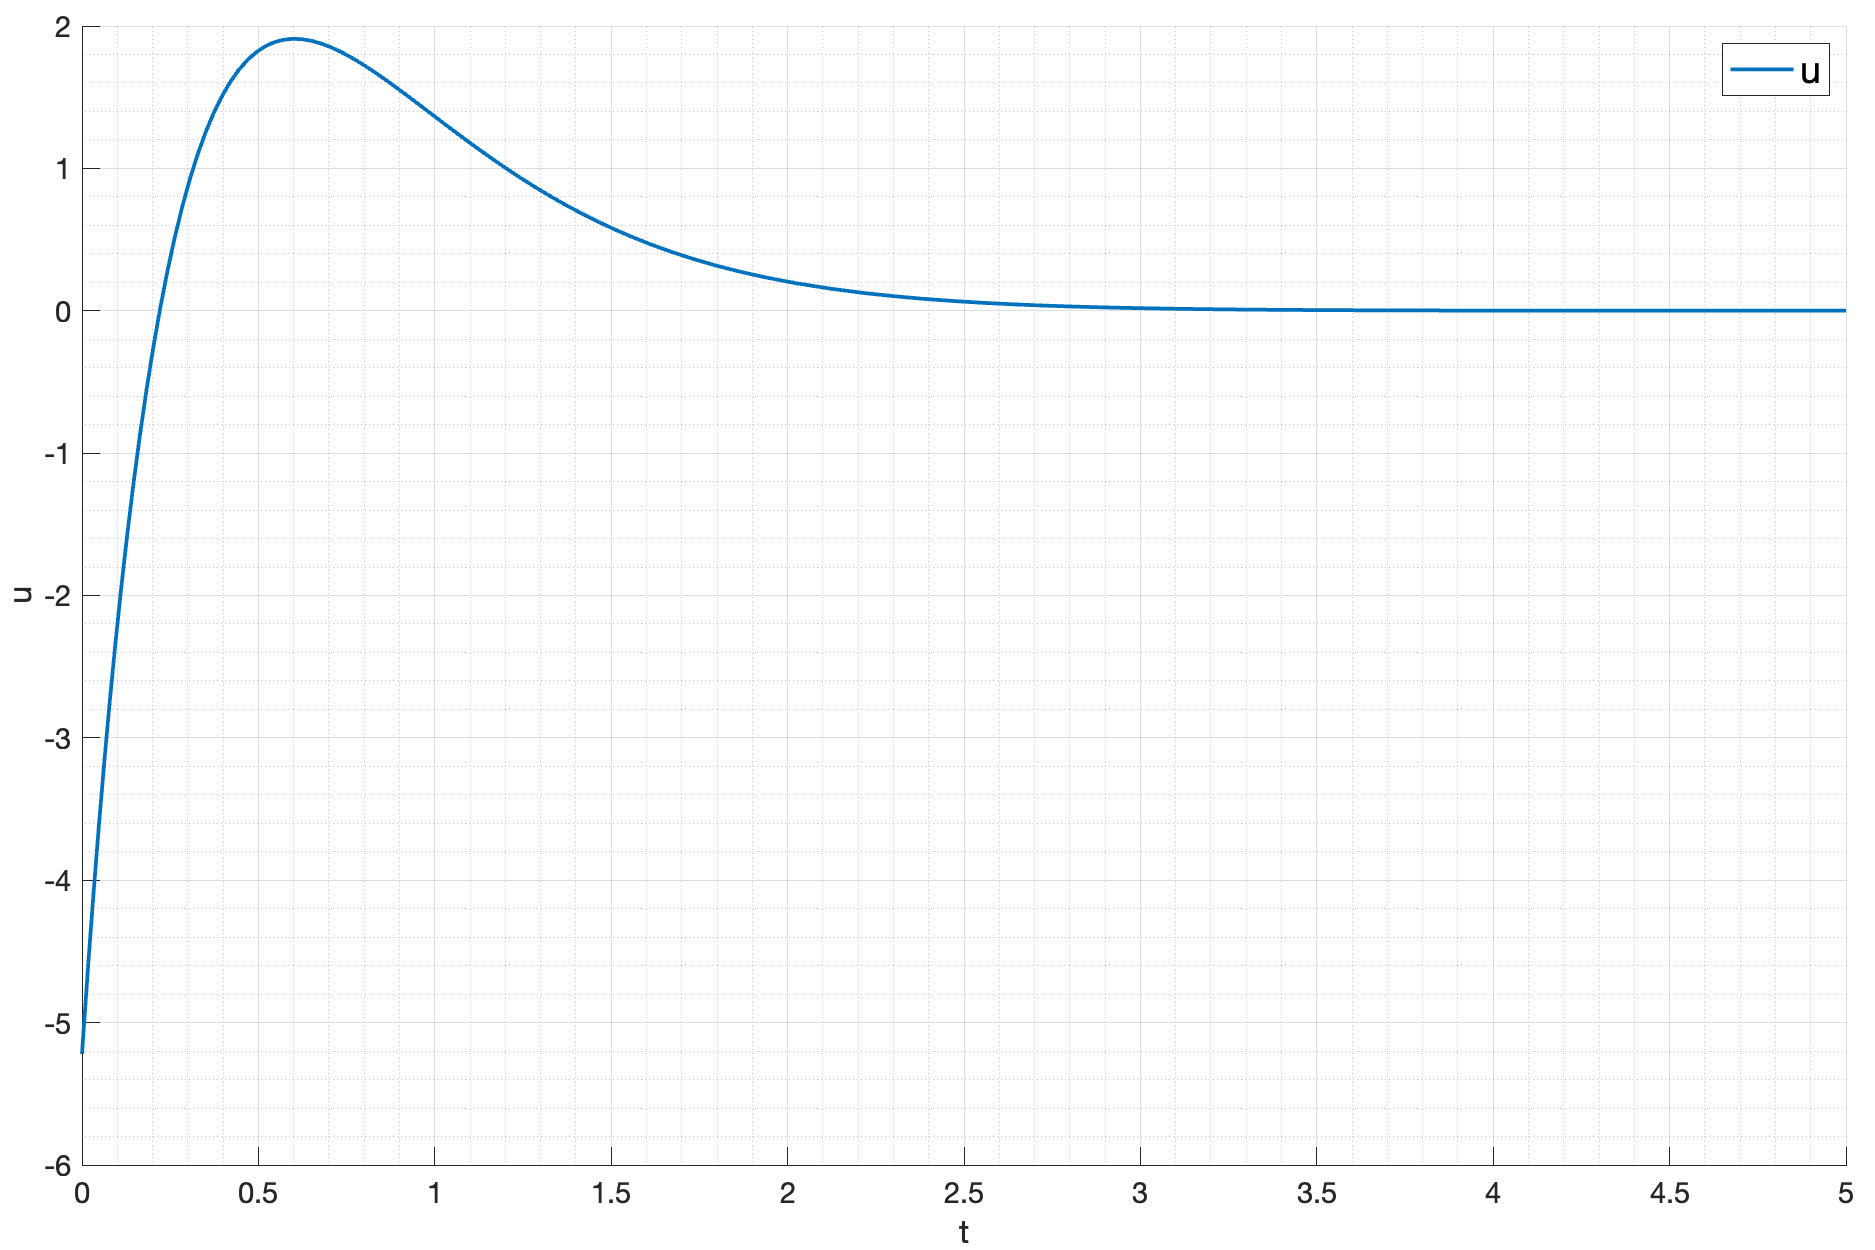
\includegraphics[width=\textwidth]{media/plots/task3_1_u.png}
    \caption{Управляющее воздействие системы с регулятором $K_1$}
    \label{fig:task3_1_u}
\end{figure}

Для системы с регулятором $K_2$ результаты моделирования представлены на рисунке \ref{fig:task3_2_x} 
(состояние системы) и \ref{fig:task3_2_u} (управляющее воздействие).

\begin{figure}[ht!]
    \centering
    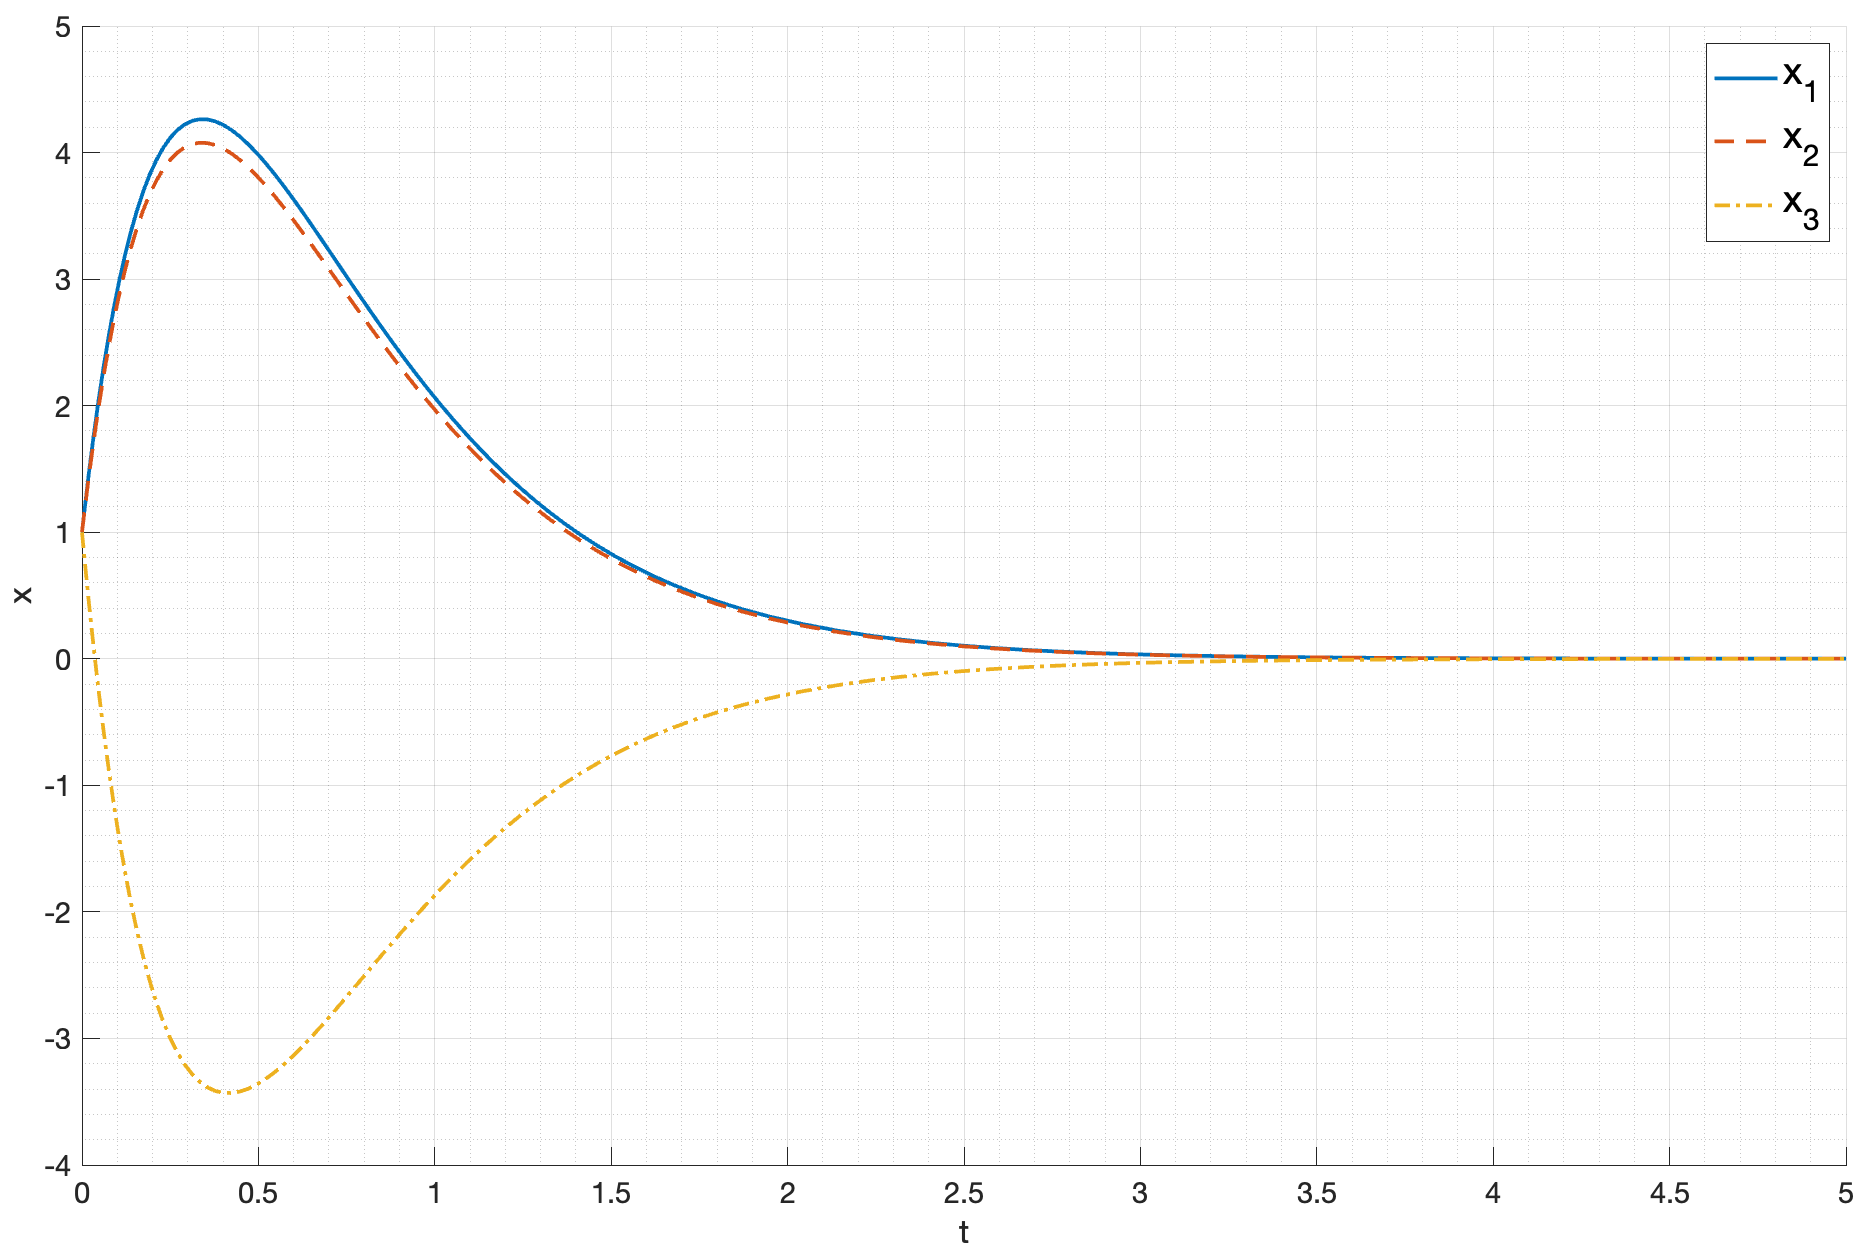
\includegraphics[width=\textwidth]{media/plots/task3_2_x.png}
    \caption{Состояние системы с регулятором $K_2$}
    \label{fig:task3_2_x}
\end{figure}
\begin{figure}[ht!]
    \centering
    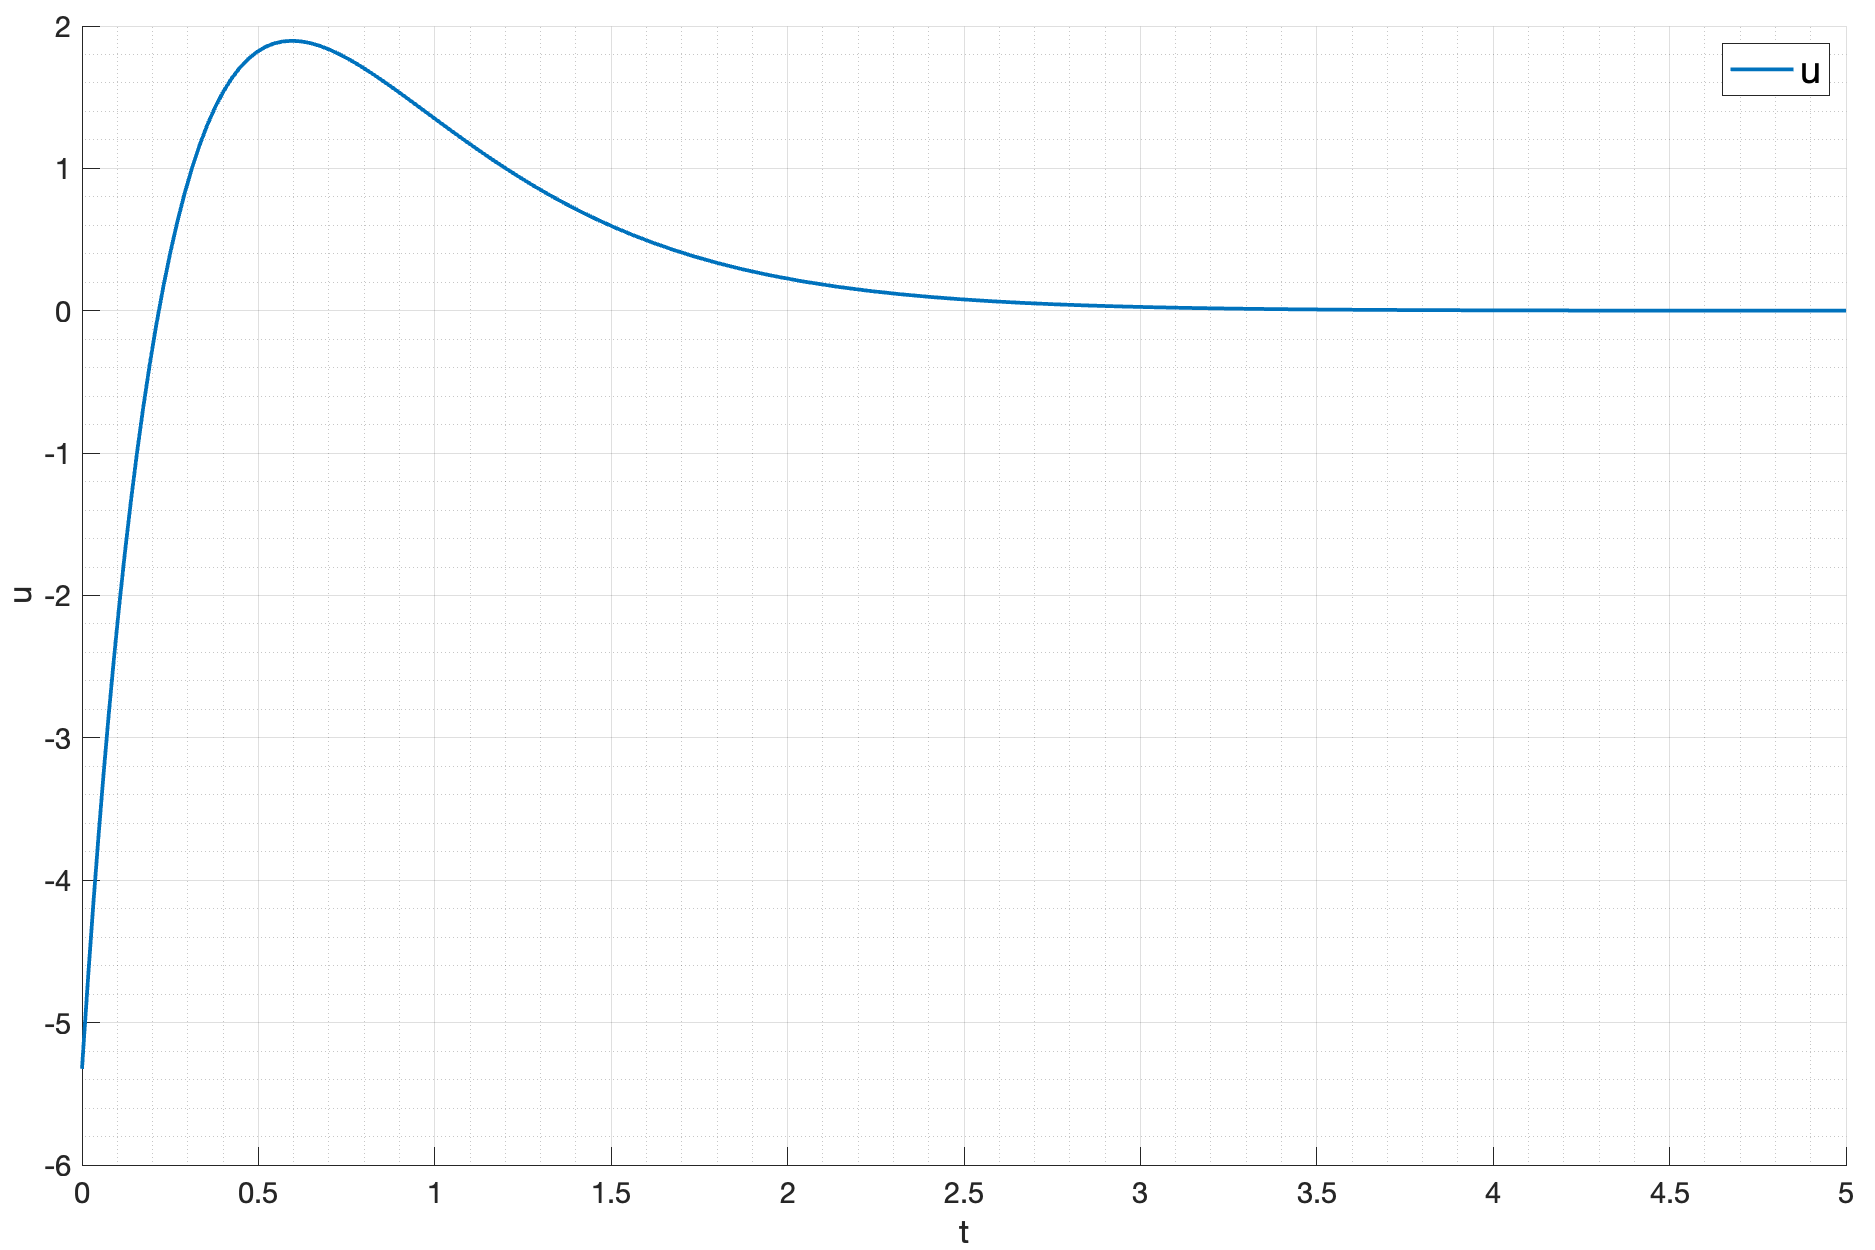
\includegraphics[width=\textwidth]{media/plots/task3_2_u.png}
    \caption{Управляющее воздействие системы с регулятором $K_2$}
    \label{fig:task3_2_u}
\end{figure}

Для системы с регулятором $K_3$ результаты моделирования представлены на рисунке \ref{fig:task3_3_x} 
(состояние системы) и \ref{fig:task3_2_u} (управляющее воздействие).

\begin{figure}[ht!]
    \centering
    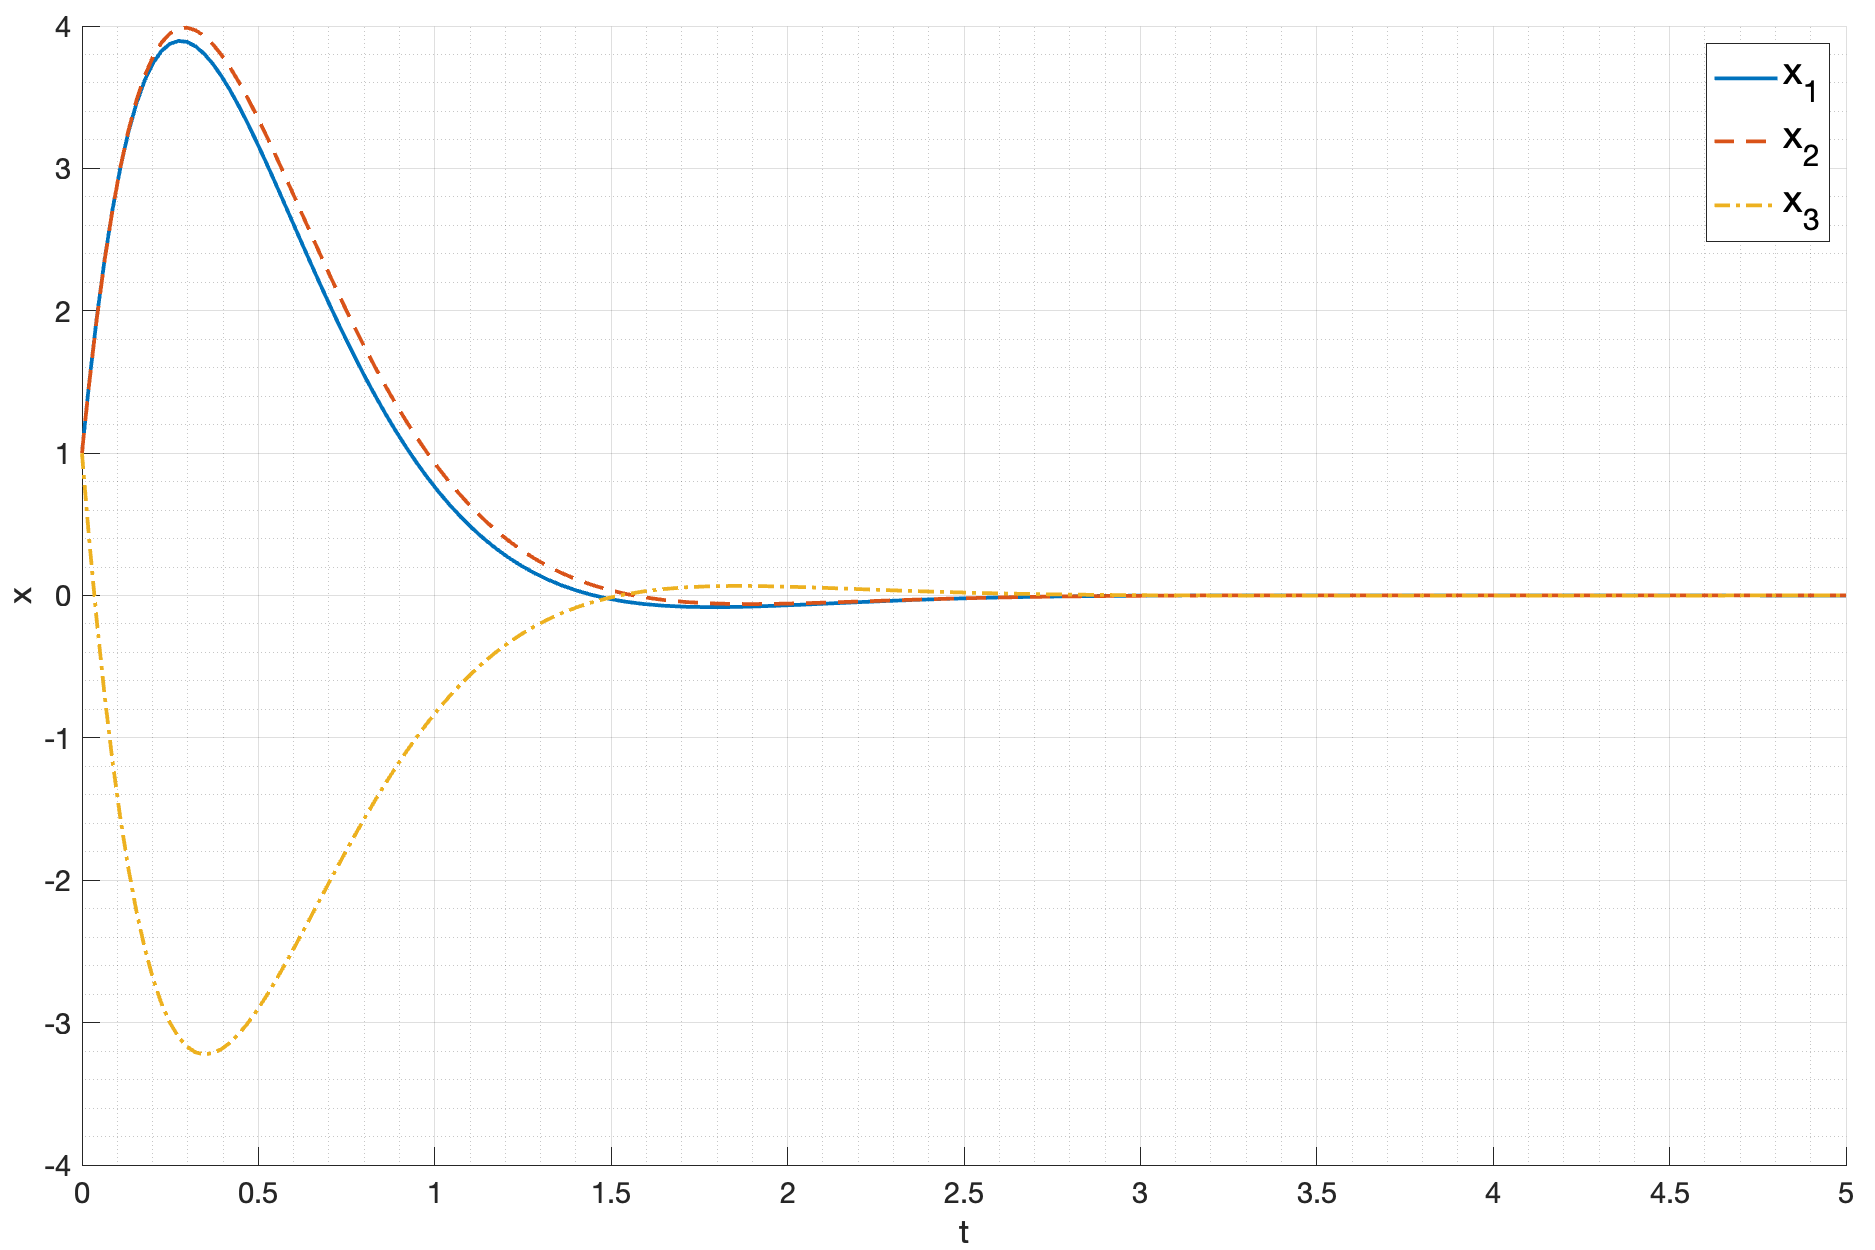
\includegraphics[width=\textwidth]{media/plots/task3_3_x.png}
    \caption{Состояние системы с регулятором $K_3$}
    \label{fig:task3_3_x}
\end{figure}
\begin{figure}[ht!]
    \centering
    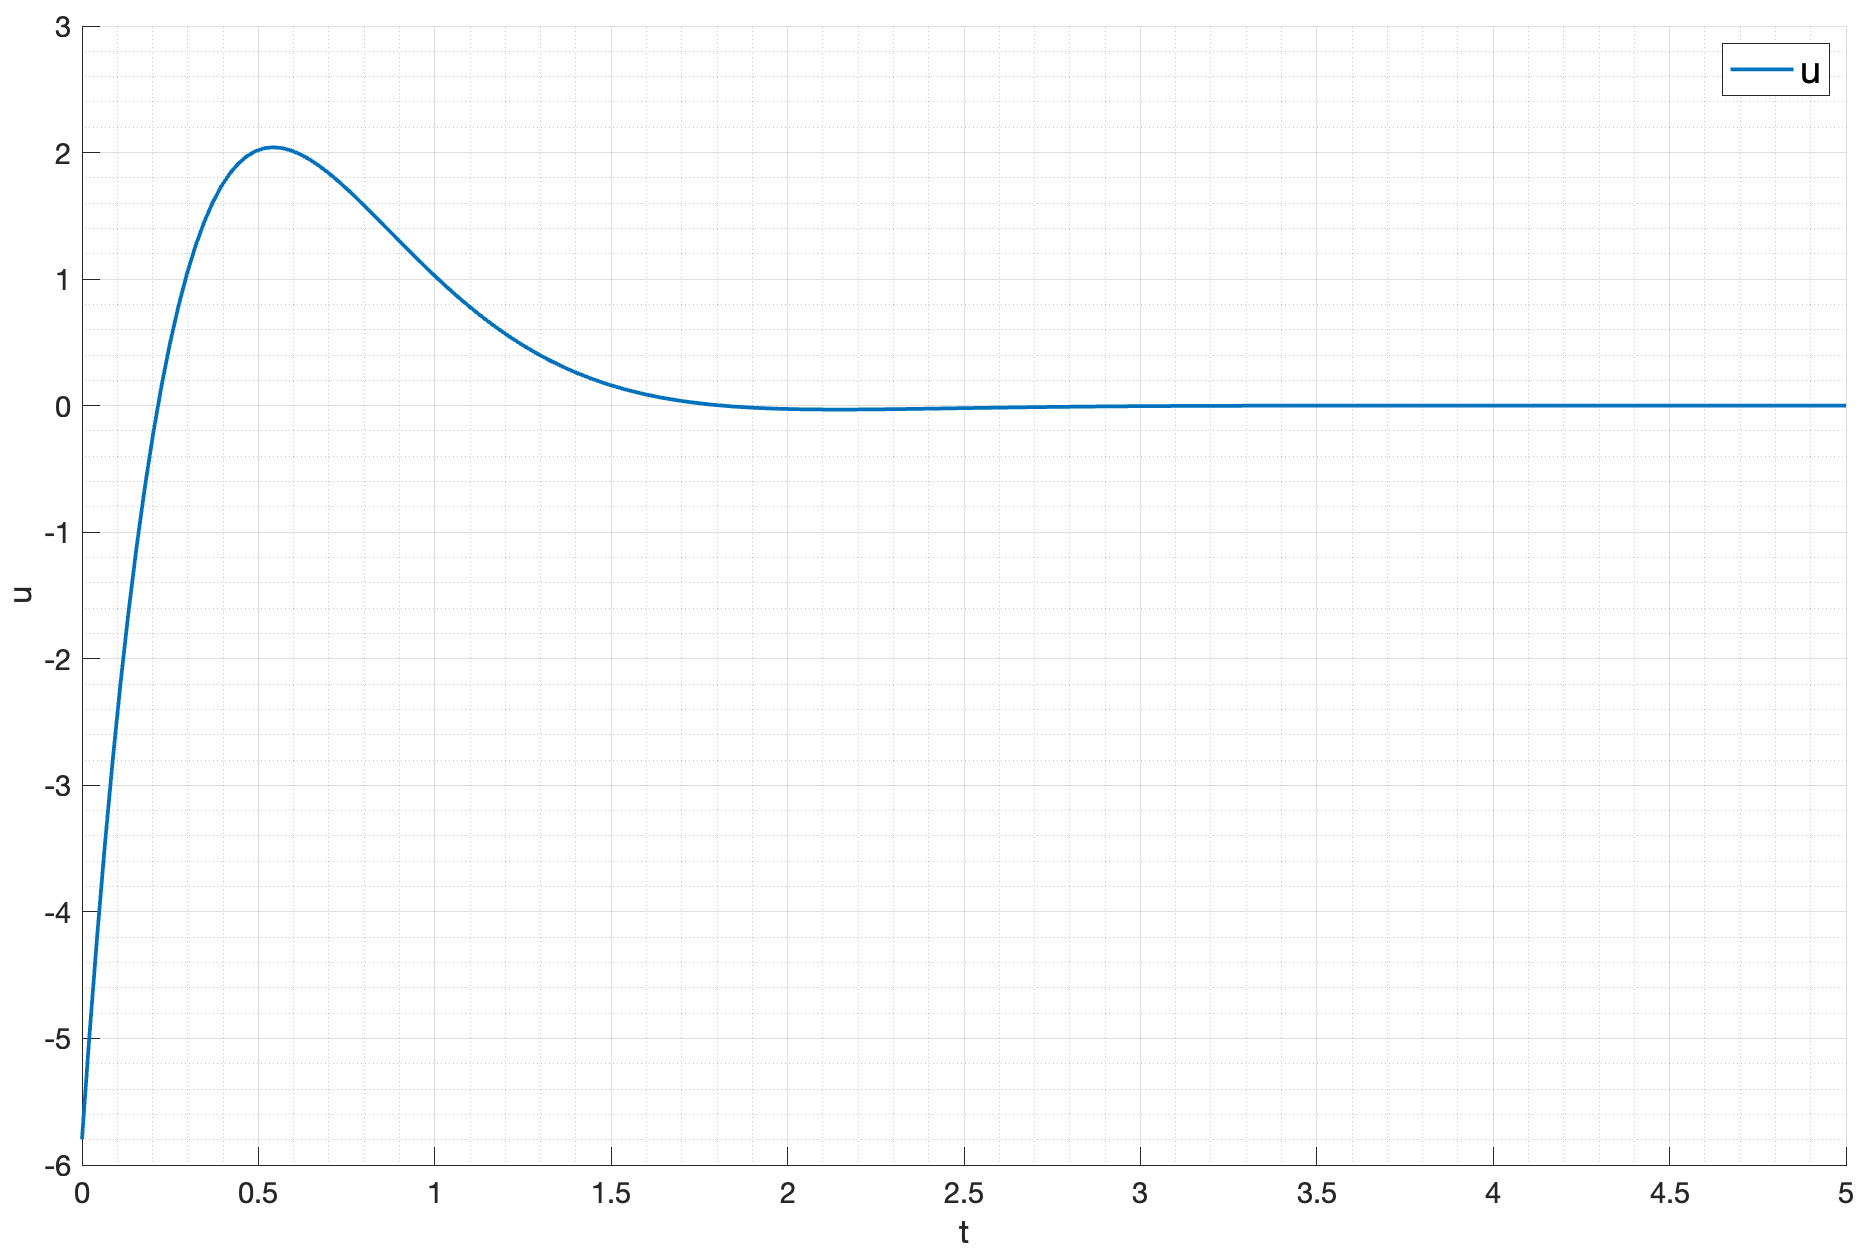
\includegraphics[width=\textwidth]{media/plots/task3_3_u.png}
    \caption{Управляющее воздействие системы с регулятором $K_3$}
    \label{fig:task3_3_u}
\end{figure}

Для системы с регулятором $K_4$ результаты моделирования представлены на рисунке \ref{fig:task3_4_x} 
(состояние системы) и \ref{fig:task3_4_u} (управляющее воздействие).
\begin{figure}[ht!]
    \centering
    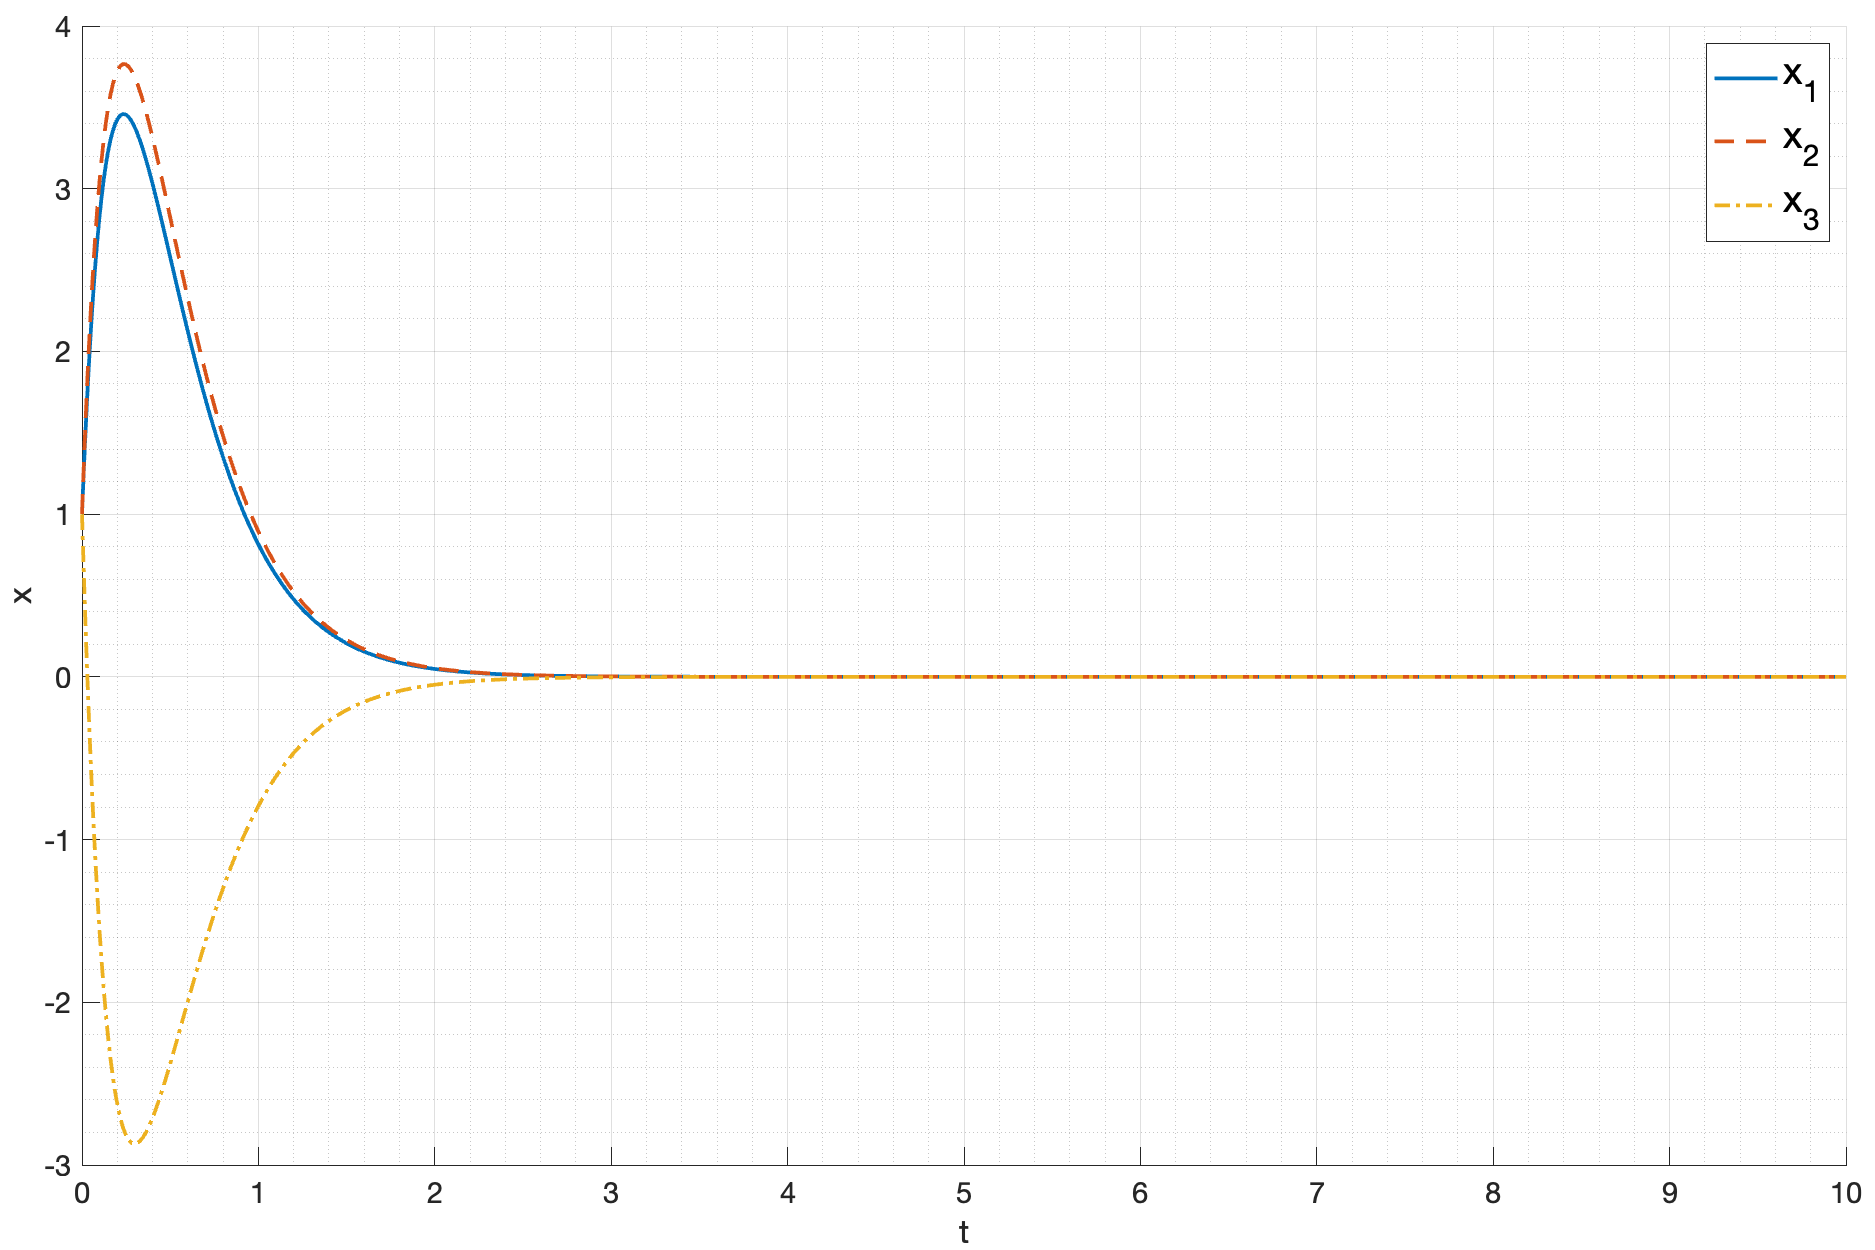
\includegraphics[width=\textwidth]{media/plots/task3_4_x.png}
    \caption{Состояние системы с регулятором $K_4$}
    \label{fig:task3_4_x}
\end{figure}

\begin{figure}[ht!]
    \centering
    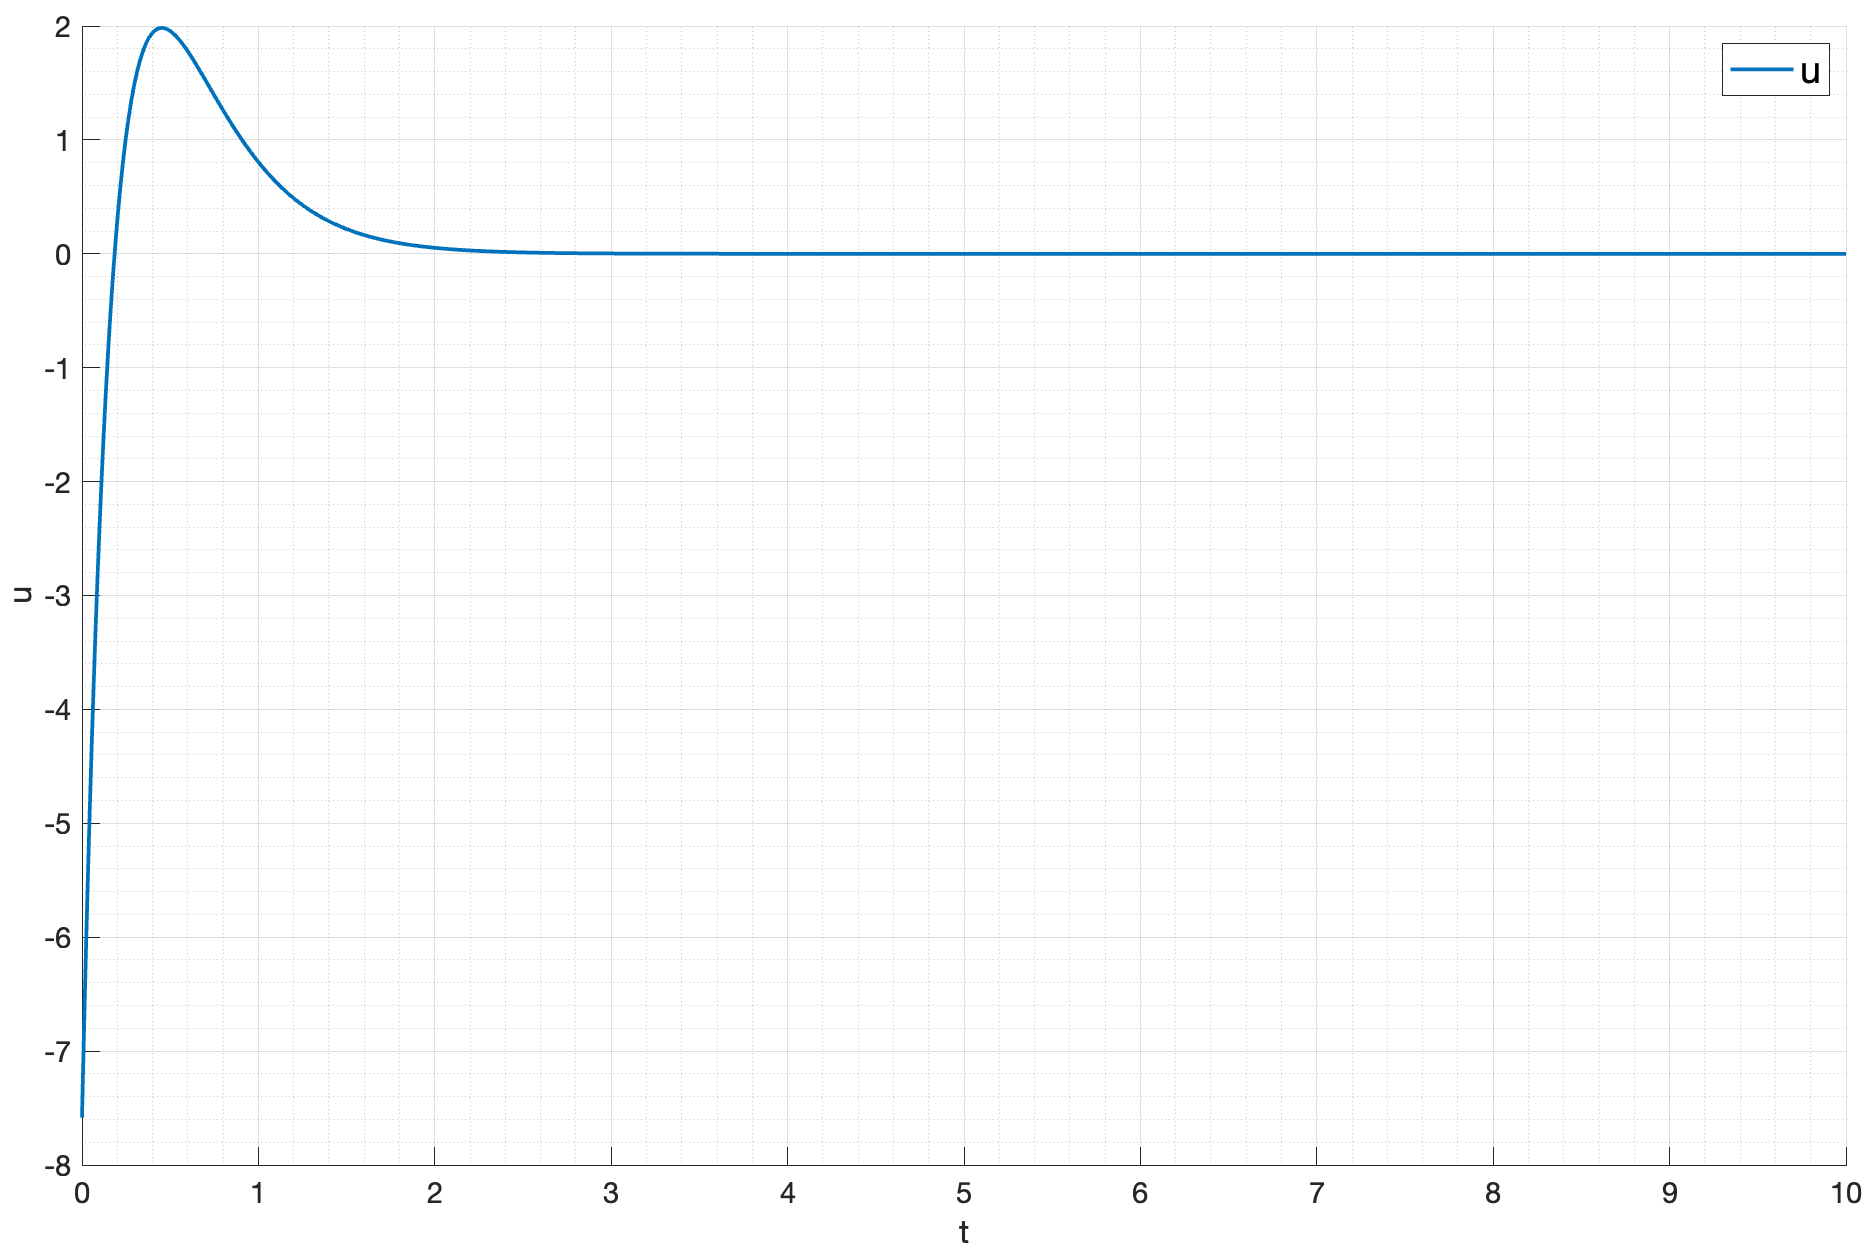
\includegraphics[width=\textwidth]{media/plots/task3_4_u.png}
    \caption{Управляющее воздействие системы с регулятором $K_4$}
    \label{fig:task3_4_u}
\end{figure}

\FloatBarrier
\subsection{Выводы}
В данном пункте был рассмотрен регулятор с качественной экспоненциальной устойчивостью, 
то есть регулятор, обеспечивающий заданное отклонение от средней траектории системы. Это наглядно 
демонстрируется на комплексной плоскости, где собственные числа системы располагаются внутри окружности,
центрированной в точке $\beta$ и радиусом $r$.
Матрица $Q$ определяет штраф на вектор состояния, а матрица $R$ -- штраф на управляющее воздействие.
При $Q = I$ система сходится быстрее к нулю, чем при $Q = 0$, 
При $R = 1$ управляющее воздействие не вызывает резких изменений в системе, аналогично 
оптимизации управления в предыдущих заданиях. 